\cotefile{12}
\scanpage{115}

% slanted
\margin{résolution, Lefschetz fort, et le cas échéant semi-simplicité}

\uline{Cor.} 5.4. Sur un corps $k$, si $X$ est lisse, séparé, de t.f., et si $F$ est \deleted{\unsure{un}} str$^{\rm t}$ spécial de poids $j$ (resp. eff$^{\rm t}$ adm. de poids $j$, si l'on admet conjecture de $\tfrac{1}{2}$simplicité), alors $R^i f_*(F)$ est de \deleted{\unsure{par}}eff$^{\rm t}$ admissible de poids entre $i+j$ et $2m+2j$, et les niveaux \unsure{corresp.dt|correspondants} de Hodge resp. $\leq 2(m-i+j),2\unsure{(m-i+j)|n-i+j}-1,\ldots,0$. Si en \unsure{$+$} $i\leq m$, on a \deleted{les niveaux} \inserted{seulement} des poids \deleted{dans la suite \unsure{des|d'ind}} $i+j,i+j+1,\ldots,2(i+j)$, \deleted{de} niveaux correspondants $\leq i+j,i+j-1,\ldots,0$.

On peut, soit procéder par dualité à partir de 5.1 et 5.2, soit reprendre \inserted{dans le cas $F$ quelc.} la dém. de 5.1 ou 5.2, en utilisant la \deleted{suite exacte de cohomologie relative} \inserted{\unsure{trivialité} de la suite spectrale de Leray}, pour se ramener au cas où $F$ est $\mathbb Q_\ell$. Dans ce cas, on peut procéder par \inserted{compactification et} résolution des singularités, pour écrire $X=\widehat X-D$, $\widehat X$ \deleted{projectif et lisse} propre et lisse et $D$ \inserted{div} à croisements normaux, et on écrit suite exacte de coh. relative (\unsure{support quelc.|supports quelc.}) pour $X,\widehat X$ et $D$, et la suite spectrale de localisation pour $H^{*}_D(\widehat X)$.

% slanted
\margin{le faire à titre de vérification de cohérence du yoga !}

6. Soit $f:X\unsure{\longrightarrow|\text{---}}S$ un morphisme de \unsure{s.f.|t.f.}, $F$ un faisceau \deleted{très spécial} \inserted{effectivement admissible} sur $X$, de poids $j$. On veut des renseignements sur \inserted{les} $R^{\unsure{\nu|n|i}}f_*(F)$, en particulier on veut qu'ils soient effectivement admissibles, de poids que nous préciserons. \deleted{Comme} \inserted{Supposons d'abord $F=\mathbb Q_{\ell X}$} pour le th. de finitude, on regarde d'abord le cas d'une immersion

% archive sheet number: 114
\scanpage{116}

\[ X\lhook\joinrel\relbar Y \]

\[ X_0\ X_1\ \cdots \]

\deleted{$X\lhook\joinrel\relbar Y$}

\[ \unsure{\mathbb Q|Q}_\ell \]

\diagram{\begin{tikzcd}[ampersand replacement=\&] X_0\arrow[r,hook,no head,"i"'] \& X\arrow[r,hook,no head,"f"'] \& Y \end{tikzcd}}

$X$ \uline{régulier}

\figure{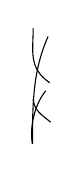
\begin{tikzpicture}[scale=.42]\draw (0,3.5) .. controls (0,2.8) and (-.15,2.3) .. (.5,1.85); \draw (.45,3.25) .. controls (.03,2.3) and (-.03,1.4) .. (-.02,0); \draw (0,1.35) .. controls (.03,1.02) and (.25,.88) .. (.53,.66); \draw (.38,1.61) .. controls (-.03,1.1) and (-.10,.35) .. (-.02,0);\end{tikzpicture}}

\[ i_!(\mathbb Q_{\ell X_0})\longrightarrow {}^{\unsure{\uparrow|t}}R i_*(\mathbb Q_{\ell X_0}) \]

\unsure{4|$\hookleftarrow$}

\textcircled{1} $X$ \uline{régulier}, $F=\mathbb Q_{\ell X}$, $f$ immersion \quad $(n=\dim\overline{f(x)})$

On peut supposer $X\longrightarrow Y$ imm. \uline{ouverte}

\diagram{\begin{tikzcd}[ampersand replacement=\&,column sep=small,row sep=small] {} \& Y'\arrow[d,"h"] \\ X\arrow[ur,hook,no head,"g"]\arrow[r,hook,no head,"f"'] \& Y \end{tikzcd}}

$Y'$ régulier, $Y'-g(X)=\deleted{\unsure{Z}}h^{-1}(Y-X)=Z$ diviseur à crois$^{\rm mt}$ norm$^{\rm x}$ \quad $Z=\sum Z_i$

\[ \deleted{\unsure{H}}\ R^*f_*(\mathbb Q_{\ell X})\Leftarrow E_2^{pq}=R^p h_*(R^qg_*(\mathbb Q_\ell)\unsure{(-1)))} \]

\[ R^qg_*(\mathbb Q_\ell)=\bigwedge^{q}\sum\mathbb Q_{\ell Z_i}=\sum_{i_1<\cdots<i_q}\mathbb Q_{\ell Z_{i_1}\cap\cdots\cap Z_{i_q}}(-q \]

\margin{$X\lhook\joinrel\relbar$}

pur de poids $2q$

\[
\begin{aligned}
E_2^{p0}=R^p h_*(\mathbb Q_{\ell\deleted{\unsure{X_0}}Y'})&\quad\text{est eff$^{\rm t}$ admissible de poids }\leq p=i\\
&\quad\text{niveau }\leq\operatorname{Inf}(p,2n-2-p\\
&\quad[\text{\unsure{au complet si|au compl. si|avec égalité si}}\ \deleted{\unsure{\leq 4p}}\ p\geq n-1]
\end{aligned}
\]

\[
\begin{aligned}
E_2^{pq}=\sum_{i_1<\cdots<i_q} R^p f_{Z_{i_1}\cap\cdots\cap Z_{i_q}*}(\mathbb Q_\ell)(-q)&\quad\text{est eff. admissible}\\
&\text{de poids }\leq p+2q=i+q\ \deleted{\leq}\leq 2n\deleted{\unsure{-2}}\\
&\text{de niveau }\leq\operatorname{Inf}(p,2n-2q-p)
\end{aligned}
\]

\[ p\deleted{\unsure{\leq}}\ 2(n\deleted{\unsure{q}}-q)\,/\,p \]

\[ \text{\textcircled{\unsure{Pds|5.e}}}\quad i+q=\boxed{\begin{aligned}p+2q&\leq 2n\deleted{\unsure{-2}}\\ q&\leq n,2n-i\end{aligned}} \]

\[
\begin{aligned}
&\text{en tous cas, poids entre }\ \text{\tikz[baseline=(a.base)]\node[draw,ellipse,inner sep=2pt](a){$\leq\deleted{\unsure{2i}}$};}\operatorname{Inf}(2i,2n-2\\
&\text{niveau }\leq\deleted{\unsure{2i-p}}\operatorname{Inf}(i,2n-2-i)
\end{aligned}
\]

\figure{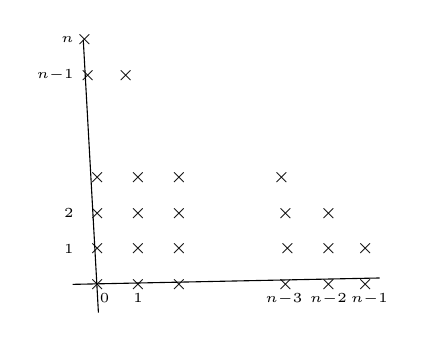
\begin{tikzpicture}[x=.52cm,y=.45cm]
\draw (-.6,0)--(6.9,.18); \draw (.03,-.8)--(-.34,6.9);
\foreach \x/\y in {0/0,1/0,2/0,4.6/0,5.65/0,6.55/0,0/1,1/1,2/1,4.65/1,5.65/1,6.55/1,0/2,1/2,2/2,4.6/2,5.65/2,0/3,1/3,2/3,4.5/3,-.23/5.9,.70/5.9,-.31/6.9}{\node[inner sep=0pt] at (\x,\y) {$\scriptstyle\times$};}
\foreach \x/\lab in {.18/0,1/1,4.56/{n-3},5.65/{n-2},6.65/{n-1}}{\node[below] at (\x,.02) {$\scriptscriptstyle\lab$};}
\foreach \y/\lab in {1/1,2/2,5.9/{n-1},6.9/n}{\node[left] at (-.34,\y) {$\scriptscriptstyle\lab$};}
\end{tikzpicture}}

\[ \begin{aligned}p&\leq n-1\\q&\leq n\end{aligned} \]

\[ \begin{aligned} &p\qquad \unsure{n+q|n-q}\\[-2pt] &\overbrace{p+q\geq n}\end{aligned} \]

\[ \begin{aligned}2(p-n+q)&=2(i-n)\qquad \unsure{2n-2}-\\ 2(n-q)-p&=\underline{2n-i}-q\end{aligned}\qquad 2. \]

% archive sheet number: 115
\scanpage{118}

\diagram{$i\leq n-1\qquad
\begin{array}{l|cccc|}\text{poids}&0&1&\hspace{3em}&2i\\\hline
\text{niveaux}&0&1&&2i\\\hline\end{array}$}

\diagram{$E_2^{i\,0}\qquad
\begin{array}{l|c|c|c|c|}\text{poids}&\unsure{0}&1&&i\\\hline
\text{niveau }\leq&0&1&&i\\\hline\end{array}$}

\diagram{$E_2^{i-1\,1}\qquad
\begin{array}{l|c|cc|c|c|}\text{poids}&2&3&&i&i+1\\\hline
\text{niveau}&0&1&&i-2&i\deleted{\unsure{+2}}\unsure{-1}\\\end{array}$}

\margin{\deleted{\unsure{car}}\quad \deleted{$p+q=i$}}

\diagram{$E_2^{\unsure{(i-2),2|i-2,2}}\qquad
\begin{array}{l|c|c|c|c|c|c|}\text{poids}&4&5&\diagup\!\diagup&i&i+1&\deleted{\unsure{2}}i+2\\\hline
\text{niveau}&0&1&\diagup&i-4&i-3&i-2\end{array}$}

\margin{\deleted{$p\leq \unsure{2}(n-1-q)$}\quad \deleted{$p+q\leq n-1$}\quad $i\deleted{\unsure{+q\leq}}$}

\diagram{$E_{\deleted{\unsure{*}}2}^{0\,i}\qquad
\begin{array}{l|c|}\text{poids}&2i\\\hline \text{niveau}&0\end{array}$}

\diagram{\tikz[baseline=(a.base)]\node[draw,ellipse,inner sep=2pt](a){$i\leq n-1$};\quad
$\boxed{\begin{array}{l|c|c|c|c|c|c|c|c|}\text{poids}&0&1&\cdots&i-1&i&i+1&\cdots&2i\\\hline
\text{niveau}&0&1&&i-1&i&i-1&&0\end{array}}$}

\diagram{\tikz[baseline=(a.base)]\node[draw,ellipse,inner sep=2pt](a){$i\geq n$};\quad
\uuline{$E_2^{i\,0}$}\quad $
\begin{array}{|c|c|c|c|c|c|}2(i-n+1)&2(i-n+1)+1&\cdots&-&\deleted{\unsure{i-1}}&i\\\hline
0&1&2&&\deleted{\unsure{i}}&2(n-1)-i\end{array}$}

\diagram{$E_2^{i-1,1}\qquad
\begin{array}{|c|c|cc|c|c|}2(i-n)+2&2(i-n)+3&&\hspace{1em}&i&i+1\\\hline
0&1&&&2n-i-2&2n-i-\unsure{1|2}\end{array}$}

\diagram{$E_2^{i-2,2}\qquad
\begin{array}{|c|c|c|c|c|c}2(i-n)\deleted{\unsure{+3}}+4&2(i-n)+\unsure{3|5}&&i&i+1&i+2\\\hline
0&1&&2n-i-2&2n-i-3&2n-i-2\end{array}$}

\diagram{$E_2^{i-3,3}\qquad
\begin{array}{|c|c|c|c|c|c|c}2(i-n)+6&2(i-n)+7&&i&i+1&i+\unsure{3|2}&i+3\\\hline
0&1&&2n-i-6&2n-i-5&2n-i-4&2n-i-3\end{array}$}

\deleted{$E$}

\diagram{$E_2^{0\unsure{;|,}i}\qquad \begin{array}{|c|}2i\\\hline 0\end{array}$}

\figure{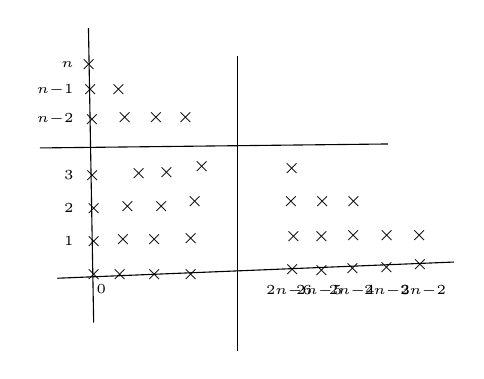
\begin{tikzpicture}[x=.44cm,y=.42cm]
\draw (0,-1.45)--(-.15,7.45); \draw (-1.05,-.11)--(10.4,.38);
\draw (-1.55,3.83)--(8.5,3.95); \draw (4.15,-2.3)--(4.15,6.6);
\foreach \x/\y in {0/0,.75/0,1.75/0,2.8/0,5.73/.14,6.58/.13,7.47/.17,8.45/.21,9.42/.30,0/1,.85/1.07,1.75/1.07,2.80/1.10,5.77/1.15,6.58/1.16,7.49/1.18,8.46/1.18,9.4/1.19,0/2,.98/2.04,1.95/2.05,2.92/2.20,5.7/2.20,6.6/2.20,7.5/2.22,-.04/3,1.30/3.05,2.10/3.07,3.12/3.25,5.72/3.20,-.05/4.69,.90/4.75,1.80/4.74,2.65/4.75,-.1/5.58,.72/5.60,-.14/6.35}{\node[inner sep=0pt] at (\x,\y){$\scriptstyle\times$};}
\foreach \y/\lab in {1/1,2/2,3/3,4.69/{n-2},5.58/{n-1},6.35/n}{\node[left] at (-.3,\y){$\scriptscriptstyle\lab$};}
\foreach \x/\lab in {.22/0,5.64/{2n-6},6.51/{2n-5},7.45/{2n-4},8.47/{2n-3},9.51/{2n-2}}{\node[below] at (\x,-.02){$\scriptscriptstyle\lab$};}
\end{tikzpicture}}

\[ \unsure{1} \]

\[
\begin{aligned}
q&=2n-i\qquad p=2(i-n)\\
E_2^{2(i-n),2n-i}&=\mathbb R^{2(i-n)}f_{Z}(\mathbb Q_\ell\\
&\phantom{={}}2(i-n)+2(2n-i)=2n
\end{aligned}
\]

% archive sheet number: 117
\scanpage{119}

20. 3. 68 \quad 1. Korrektur

Lecture Notes in Mathematics

A collection of informal reports and seminars

Edited by A. Dold, Heidelberg and B. Eckmann, Zürich

41 \hfill\rule{.67\linewidth}{1.1pt}

Local Cohomology

A Seminar given by A. Grothendieck

Notes by R. Hartshorne

1967 \hfill\rule{.67\linewidth}{1.1pt}

% crop-candidate: scan 119
\figure{
\begin{tikzpicture}[x=.72cm,y=.72cm,line cap=round,line join=round]
\draw[thick] (0,0) ellipse (.57 and .75);
\fill (0,0) ellipse (.31 and .47);
\node[text=white,inner sep=0pt] at (0,-.06){\large J};
\node[text=white,inner sep=0pt] at (0,.04){\Large S};
\node[rotate=78,inner sep=0pt] at (-.44,.11){\tiny\unsure{ALLE}};
\node[inner sep=0pt] at (0,.60){\tiny\unsure{ZEIT}};
\node[rotate=-80,inner sep=0pt] at (.43,.11){\tiny\unsure{WACH}};
\node at (0,-.58){\tiny\unsure{1842}};
\foreach \s in {-1,1}{\begin{scope}[xscale=\s]\draw[thick] (.24,-.72).. controls (.21,-.95) and (.47,-.98)..(.45,-.80) (.33,-.67).. controls (.58,-.72) and (.76,-.10)..(.68,.50); \draw (.50,.45)..controls (.85,.55) and (.59,.96)..(.46,.78)..controls (.38,.63) and (.68,.63)..(.56,.77); \draw (.09,.75)..controls (.10,.86) and (.13,.91)..(.27,.95)..controls (.38,1.06) and (.15,1.09)..(.11,.99);\end{scope}}
\draw[thick] (-.12,1.01) rectangle (.14,1.10);
\draw[very thick] (-.24,1.12)--(.22,1.12)..controls (.36,1.70) and (.12,1.87)..(-.10,1.86)--(-.18,1.90)--(-.17,1.73)--(-.38,1.48)--(-.32,1.42)--(-.09,1.52)..controls (.03,1.62) and (-.02,1.39)..(-.20,1.29)--cycle;
\draw (-.13,1.68) circle (.025); \draw (-.20,-1.03)..controls (.02,-1.00) and (-.05,-1.16)..(.20,-1.03);
\end{tikzpicture}}

Springer-Verlag $\cdot$ Berlin $\cdot$ Heidelberg $\cdot$ New York

% archive sheet number: 118
\scanpage{120}

\diagram{\tikz[baseline=(a.base)]\node[draw,ellipse,inner sep=2pt](a){$i\geq n$};\quad
$\boxed{\begin{array}{l|c|c|c|c|c|c|c|c|c}
\text{poids}&2(i-n)+2&2(i-n)+3&2(i-n+4)&\raisebox{-.6ex}{$\times$}&i&i+1&i+2&\cdots&2n\\\hline
\text{niveau}&0&1&2&&\substack{2n-i\\-2}&2n-i-1&2n-i-2&\text{---}&0
\end{array}}$}

\figure{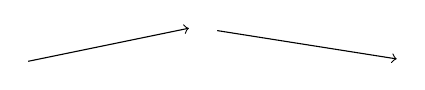
\begin{tikzpicture}[x=.6cm,y=.6cm]\draw[->] (0,0)--(3.4,.7);\draw[->] (4,.65)--(7.8,.05);\end{tikzpicture}}

\[
\begin{aligned}
&\text{poids }\underline{2n}\ \text{intervient avec }\deleted{\unsure{R^{2n}}},\quad
E_2^{2(i-n),2n-i}=\sum R^{2(i-n)}f_{\underbrace{Z_{\alpha_1}\cap Z_{\alpha_2}\cdots\cap Z_{\alpha_{2n-i}}}_{\dim\,i-n}}(\mathbb Q_\ell)(-2n+i)\\
&\qquad 2n-i\leq n\leq i\qquad\qquad n-(2n-i)=i-n\\
&\hspace{9em}2(i-n)+2(2n-i)=2n
\end{aligned}
\]

\diagram{$\boxed{\begin{array}{l|c|c|c|c|c|c|c|c|cc}
i&0&1&\cdots&n-1&\unsure{n|-}&n+1&\cdots&2n-1&\deleted{\leq 2n}&\leq 2n-1\\\hline
\text{niveau}&0&1&\cdots&n-1&n-1&n-2&\cdots&0&&\leq n-1\\\hline
\text{poids }\leq&0&2&&2n-2&2n,&2n&2n&2n&&\leq 2n
\end{array}}$}

\[ \boxed{\begin{aligned}\text{poids}&\leq 2\operatorname{Inf}(\deleted{\unsure{2}}i,\deleted{\unsure{2}}n)\\
\text{niveau}&\leq\operatorname{Inf}(i,n-1)\end{aligned}} \]

Si $F$, \deleted{\unsure{str|str$^{\rm t}$}} spécial de poids $i$

\[ \begin{aligned}\text{poids}&\leq 2\operatorname{Inf}(i,n)+j\quad ?\\
\text{niveau}&\leq\operatorname{Inf}(i,n-1)+j\end{aligned} \]

\deleted{\textcircled{\unsure{2|2\textsuperscript{o}}} $f$ \unsure{séparé de t.f.}, $F=\mathbb Q_{\ell X}$}

% slanted
\margin{Cas général relatif en \unsure{gardant} \unsure{même} $n$}

\diagram{\begin{tikzcd}[ampersand replacement=\&] X\arrow[d,"f"]\\Y\ni y \end{tikzcd}}

\[ n\deleted{\unsure{d_y|=y}}=d_y(f)=\underset{\substack{x\in X\\\text{t.q. }f(x)\in\operatorname{Sp}\mathcal O_{Y,y}}}{\operatorname{Sup}}
\left[\deg \mathrm{tr}\,[k(x):k(f(x))]+{}\deleted{\unsure{d|{+}}}\dim\left(\overline{f(x)}\big/ \unsure{y\ d_y|y}\right)\right. \]

\margin{au vois. de \deleted{\unsure{$x$}} $y$}

\[ \boxed{\begin{aligned}\text{poids}&\leq 2\operatorname{Inf}(i,n)+j\\
\text{niveau}&\leq\operatorname{Inf}(i,n)+j\end{aligned}}\quad ? \]

\margin{peut se remplacer par $n-1$ si $f$ est \deleted{à fibres \unsure{non}} \unsure{de dim|ou dim} $\leq n-1$ ?}

% archive sheet number: 119
\scanpage{122}

2) $F$ \deleted{\unsure{$=\mathbb Q_{\ell X}$}} strictement spécial\inserted{ de poids $j$}, $X$ régulier.

On peut supposer $F=R^dp_*(\mathbb Q_{\ell X'})$, \fbox{$p$ de dim relative $d$}

\diagram{\begin{tikzcd}[ampersand replacement=\&,column sep=large,row sep=large,execute at end picture={\draw[rounded corners=2pt] ([xshift=3mm,yshift=5mm]xp.east) rectangle ([xshift=4mm,yshift=-7mm]yp.east);}]
|[alias=xp]|X'\arrow[r,hook,no head,"f'"]\arrow[d,"p"'] \& |[alias=yp]|Y'\arrow[d,"q"]\\
X\arrow[r,hook,"f"'] \& \deleted{\unsure{X}}Y
\end{tikzcd}}

On a alors

\[ \unsure{\mathbb R|R}^*(fp)_*(\mathbb Q_{\ell X'})\Longleftarrow E_2^{pq}=\mathbb R^p f_*(R^q\unsure{g|p|\varphi}_*(\mathbb Q_\ell)) \]

suite spectrale qui \uline{dégénère} par Deligne, donc $R^if_*(F)=R^if_*(R^j g_*(\mathbb Q_{\ell\unsure{X|X'}}))$ est un \uline{morceau} de $R^{i+j}(fp)_*(\mathbb Q_{\ell X'})$

\[ \text{Or}\qquad R^*(fp)_*(\mathbb Q_{\ell X'})\Longleftarrow \deleted{\unsure{E}}E_2^{pq}=R^p q_*(R^q f'_*(\mathbb Q_{\ell X'})) \]

Or $Y'$ est de dim \deleted{\unsure{$n+j$}} $n'\leq\text{\tikz[baseline=(a.base)]\node[draw,ellipse,inner sep=1pt](a){$n+j$};}$

\[
\begin{aligned}
\text{donc}\qquad R^q f'_*(\mathbb Q_{\ell X'})&\quad\text{est effectif de poids }\leq 2\operatorname{Inf}(\deleted{\unsure{2}}q,\deleted{\unsure{2}}n+\deleted{\unsure{2}}j)\\
&\text{de niveau }\leq\operatorname{Inf}(q,n+j-1)
\end{aligned}
\]

$\unsure{q|g}$ est de dim relative $\leq$

\deleted{\unsure{On prend} $p+q=i+j$}

\deleted{\unsure{avec} $p+q\unsure{=}$} $E_2^{pq}$ de poids $\leq$

% archive sheet number: 121
\scanpage{125}

\uline{Dévissage de $\mathbb Q_\ell$-faisceaux}

\deleted{Un faisceau}

Un $\mathbb Q_\ell$-faisceau \deleted{\unsure{est dit}} \inserted{$F$} sur $X$ est dit \uline{admissible} \inserted{de type $\leq d$} s'il satisfait la condition suivante :

$\forall x\in X$, existe voisinage ouvert $U$ de $x$ dans $\overline{x}$ et filtration \inserted{finie} de $F|U$ par des ss-faisceaux \deleted{\unsure{$F^i$}} tels que les $\operatorname{gr}^i(F|U)$ soient isomorphes à un \deleted{``facteur''} \inserted{quotient \inserted{\unsure{ess. constant|ens. constant|en. constituants}} d'un sous-objet ess. constant} de un faisceau de la forme $R^n g_*(\deleted{\unsure{\mathbb Q_{\ell V}}}\mathbb Q_\ell)$, où $g:V\unsure{\longrightarrow|\text{---}}U$ est un morphisme \uline{projectif}, \deleted{\unsure{et}} \uline{lisse}, à fibres connexes \inserted{de dim $\leq d$}.

% slanted
\margin{``ess. constant'' signifie : faisceau de \unsure{Steenrodien|Steenro-dien} \unsure{!|''}}

[Se vérifie fibre par fibre, + $F$ est ``constructible'']

\deleted{Ceci dit que $F$ est \unsure{admis. si|admissible}} \inserted{\unsure{vrai} pour \uline{fibres} \uline{géom}}

\uline{Lemme} 1 \quad Les \deleted{\unsure{fai}} $\mathbb Q_\ell$-faisceaux admissibles de type $\leq d$ forment une sous-catégorie abélienne \deleted{\unsure{exacte} et épaisse (stable par} \inserted{épaisse de la catégorie des $\mathbb Q_\ell$-faisceaux constructibles} \deleted{noyau, conoyau, extension) de la catégorie des}

\deleted{\unsure{2}} (i) Stable par ss-\deleted{\unsure{fais|faisc.}}objet et objet quotient.

En effet, si $F|U$ est muni d'une filtration $d$-spéciale, \inserted{et si $G|U$ est ess. constant,} alors la filtration induite sur $G$ resp $(F\unsure{\vert U|\cap U})/G$ est $d$-spéciale. \deleted{\unsure{car $H$ de}}

(ii) Stable par extensions : trivial.

\uline{Lemme} 2 \quad \uline{Images inverses} \qquad trivial.

% archive sheet number: 124
\scanpage{127}

\uline{Lemme} \deleted{2}3 \quad Soit $f:X\unsure{\text{---}|\longrightarrow}Y$ un morphisme \inserted{compactifiable} de type fini, de dim relative $\leq d'$, $F$ un $\mathbb Z_\ell$-faisceau admissible de type $\leq d$ sur $X$, alors pour \deleted{\unsure{tt|tout}} $i$, $R^i_!f(F)$ sur $Y$ sont admissibles de type $\leq d+d'$

\margin{$\Big\downarrow$}

On peut supposer $Y=\operatorname{Sp}k$, $k$ un corps.

Récurrence sur $d+d'$, trivial si $d'\leq0$. Supposons $d+d'>0$, et le th. démontré pour les \deleted{\unsure{$d'$}} \inserted{$\delta'<d'$}.

Soit $U\subset X$ \inserted{ouvert} lisse sur $K$ et dense dans $X$, et \inserted{que $F|U$ ait une filtration $d$-admissible.} [NB. on est obligé dans la déf. plus haut d'admettre une extension radicielle sur la base.] et soit $Z=X-U$.

On a

\[ \unsure{\mathbb R|R}^{\unsure{-|i}}_! f_U(F|U)\longrightarrow \mathbb R^{-}_!f_*(F)\unsure{\text{---}|\longrightarrow}R^{-}_!f_{\unsure{Z|Y}*}(F|Y) \]

ce qui ns ramène au cas de $f_Z$ et $f_U$ grâce aux lemmes 1 et 2 ; le cas de $f_Z$ est contenu dans l'hyp. de réc, et \deleted{\unsure{alors}} \unsure{pour|donc} le cas \deleted{\unsure{de}} où $X$ est lisse sur $k$ et a une filtration $d$-admissible.

Par dévissage et le lemme 1 \deleted{\unsure{de}} on peut supposer que $F$ est un quotient \inserted{ess. const.} d'un

% archive sheet number: 126
\scanpage{129}

sous-module \inserted{\unsure{ess. const.|ens. const.|en. const.}} d'un $R^m g_*(\mathbb Q_\ell)$, $g:V\unsure{\text{---}|\longrightarrow}U$ un morphisme \uline{projectif} de dim \inserted{relative} $\leq d$. On a donc des suites exactes

\[
\begin{aligned}
0&\longrightarrow \underset{\diagup}{G}\mathrel{\text{---}} R^{\unsure{m|n}}g_*(\mathbb Q_\ell)\mathrel{\text{---}}H\mathrel{\text{---}}0\\
0&\mathrel{\text{---}}\underset{*}{I}\mathrel{\text{---}}\underset{*}{G}\mathrel{\text{---}}F\longrightarrow 0
\end{aligned}
\]

et \deleted{\unsure{une}} \inserted{de} nouvelles applications du lemme 2 nous \unsure{ramène|ramènent} au cas de $I$ et $G$, $\unsure{\mathbb R|R}^{\unsure{-|n}}f_*(F)$ lorsque \deleted{$I,G$} $F$ ess. const. $\subset R^{m}g_*(\mathbb Q_\ell)$. Pour continuer, il faut utiliser le ``th.'' \uline{de complète réductibilité} pour nous \unsure{ramener|soumis} au cas où $F$ est de la forme $R^m g_*(\mathbb Q_\ell)$

on doit donc examiner le cas

\[ R^p_! f_*(R^q g_*(\mathbb Q_\ell))\qquad p,q\geq0 \]

\deleted{\unsure{1\textsuperscript{o})|b)} Cas $m=0$. Nous procédons par réc. \uline{descendante} sur $p+q$ \deleted{\unsure{suivant}}, en supposant que c'est vrai \unsure{pr|pour} $(p',q')$ si $p'>p$ \uuline{ou} $q$}

% archive sheet number: 128
\scanpage{131}

De plus, procédant par récurrence sur $d+d'$, et utilisant une \uline{factorisation d'Artin} de $U$ [ce qui est loisible, car on peut prendre $U$ petit], on est ramené au cas où $U$ est de \uline{dim 1}.

Alors la suite exacte pour $\deleted{\unsure{g}}fg$, \deleted{\unsure{se}} compte tenu de $R^0_!f(R^{\unsure{q|?}} g_*(\mathbb Q_\ell))=0$, se réduit à \deleted{\unsure{deux}} suites exactes courtes

\[
\begin{aligned}
0\mathrel{\text{---}}R^2_!f_*(R^{n-2}g_*(\mathbb Q_\ell))&\mathrel{\text{---}}\unsure{R^n|R^-|R^n_!}\unsure{(gf)_*|(gf)_{-}}(\mathbb Q_\ell)\mathrel{\text{---}}R^1_! f_*(R^{n-1}g_*(\mathbb Q_\ell))\\[-2pt]
&\hspace{17em}\downarrow\\[-2pt]&\hspace{17em}0
\end{aligned}
\]

donc par lemme 1 on est ramené à vérifier que $R^{\unsure{n|-}}_!\overset{\inserted{h}}{(gf)}_{\unsure{*|!}}(\mathbb Q_\ell)$ est spécial. Or utilisant la résolution des singularités pour $V$, on a $V=\widehat V-Z$, $\widehat V$ projectif et lisse sur $k$, d'où

\[ \mathbb R^{n-1}_! h_Z(\mathbb Q_\ell)\longrightarrow R^n_!\widehat h(\mathbb Q_\ell)\longrightarrow R^{\unsure{n|-}}_!\widehat h(\mathbb Q_\ell) \]

% archive sheet number: 130
\scanpage{133}

et \deleted{\unsure{$R$}} par lemme 1 il suffit de regarder les \uline{extrêmes}. Celui de droite est O.K. \deleted{\unsure{comme}} par \uline{définition}, celui de gauche par hyp de récurrence. \quad O.K.

\uline{Proposition} \uline{4} \quad Soit $i:U\unsure{\text{---}|\longrightarrow}X$ une immersion ouverte, \inserted{avec $X$ excellent, \inserted{de dim $\leq d$},} $F$ un \deleted{\unsure{fais}} $\mathbb Q_\ell$-faisceau \deleted{\unsure{$d$}}$d'$-admissible. Alors les $R^{\unsure{n|-}}i_*(F)$ sont $(d+d'\deleted{\unsure{+2}}\unsure{-1})$-\deleted{\unsure{ad}}admissibles.

\deleted{En effet, soit \inserted{\unsure{de façon qu'on}} $V\underset{j}{\subset}U$, $V$ dense dans $U$, tel que $V$ régulier.} \inserted{Récurrence sur $d+d'$, trivial si $d+d'=0$ car $d=0,d'=0$. Supposons $d+d'>0$, et \deleted{\unsure{soit}} fait si $\delta+\delta'<d+d'$}

On peut supposer $X$ affine donc noeth, et par réc. noeth., \deleted{\unsure{supposons}} le th est démontré pour les $Y\subset X$ fermés, $Y\neq X$, et $X\neq\varnothing$

Soit alors $V\underset{j}{\subset}U$ ouvert dense de $U$, régulier, alors

\diagram{\begin{tikzcd}[ampersand replacement=\&,column sep=small,row sep=small] {} \& Q^*\arrow[dl]\\ F\arrow[rr,no head] \& {} \& \mathbb R j_*F\arrow[ul]\end{tikzcd}}

où $Q$ est concentré sur $Z\cap U$, $Z=\overline{U-V}$ \uline{\unsure{vu|pris}} dans $X$, donc $\neq X$. Donc on est ramené à prouver que les $\mathbb R^n i_*(\mathbb R j_*(F))$ et $\mathbb R^n i_*(Q^*)$ sont admissibles. pour le

% archive sheet number: 132
\scanpage{135}

lemme 1 et l'hyp. de récurrence, OK. pour $\mathbb R^{\unsure{n|-}}i_*(Q^*)$. Quant à $\deleted{\unsure{D}}\mathbb R^ni_*(\mathbb R j_*(F))$ c'est aussi $\mathbb R^n(ij)_*(F)$, ce qui nous ramène au cas où $U$ est \uline{régulier}. Alors par \uuline{résolution}, on a $i=fi'$, avec $f$ projectif, $X'$ régulier, $i'$ une immersion ouverte à complémentaire un diviseur à croisements normaux

\diagram{\begin{tikzcd}[ampersand replacement=\&,column sep=large,row sep=small] {} \& X'\arrow[d,"f"]\\ U\arrow[ur,hook,"i'"]\arrow[r,hook,no head,"i"'] \& X \end{tikzcd}}

\[ \text{Alors}\qquad R^*fi'_*(F)\Longleftarrow \mathbb R^p f_*(R^q i'_*(F)) \]

et cela nous ramène \inserted{par le lemme 3} au cas où \deleted{\unsure{$\mathbb Q_\ell$} $X$} $X-U$ est un diviseur à croisements normaux. \uuline{Lorsque} $F=\mathbb Q_\ell$, on gagne alors par des calculs explicites \inserted{(th. de \uuline{pureté}).} On va ramener le cas général à celui-ci, en compactifiant $V\deleted{\unsure{/X}}$ en \deleted{\unsure{$X$}}, $g:Y\unsure{\text{---}|\longrightarrow}X$ morphisme projectif (pas lisse a priori), où $F$ est un facteur direct de $\mathbb R^nf_*(\mathbb Q_\ell)$ ; \inserted{on peut supposer dim rel. $g\leq d'$ ;}

\diagram{\begin{tikzcd}[ampersand replacement=\&,column sep=large,row sep=small]
V\arrow[r,hook,no head,"\unsure{d|j}"]\arrow[d,"f"'] \& \widehat Y\arrow[d,"g"]\\
U\arrow[r,hook,no head,"i"'] \& X
\end{tikzcd}}

On peut supposer $F=\mathbb R^n f_*(\mathbb Q_\ell),=\mathbb R^n g_*(\mathbb Q_\ell)|U$. Par des dévissages faciles, utilisant lemme 3 on est ramené au cas où $d'=1$\inserted{ et $f$ à fibres géom. conn.}. Alors la suite spectrale pour $if$ est

% slanted
\margin{\uline{développer}}

% archive sheet number: 134
